% !TeX root = ../../../master.tex

\subsection{Benutzerkonto}
\label{ssec:Benutzerkonto}

Um einem Benutzer der Anwendung die Möglichkeit zu bieten sein Passwort zu ändern, wurde eigens hierfür ein eigener Bereich implementiert.
Der Benutzer kann dies über das Icon \faUser[regular]\xspace in der Navigationsleiste dort hin navigieren.
\abb \myRefGeneral{fig:AccountImplement} zeigt das Benutzerkonto. \newline
Der Benutzer sieht in der Kartenansicht mit dem Icon \faUser[regular]\xspace seinen Benutzernamen (hier: admin).
Er kann sein Passwort selbstständig ändern.
Dadurch wird Anforderung~\hyperref[Anf:A4]{A4}, die Möglichkeit zur Passwortänderung, erfüllt.\newline
Ferner kann er über den Button \jinline|Show Published Surveys| wieder auf das Result-Dashboard navigieren (siehe Kap. \vref{ssec:ResultDashboardImplement}).
Über den Button \jinline|Show Survey Masters| kann der Benutzer auf seine Umfrage-Dashboard gelangen (siehe Kap. \vref{ssec:UmfrageDashboard}).
Wahlweise kann der Benutzer auch über die Navigationsleiste die zuvor genannten Bereiche ansteuern.

\begin{figure}[hp]
	\centering
	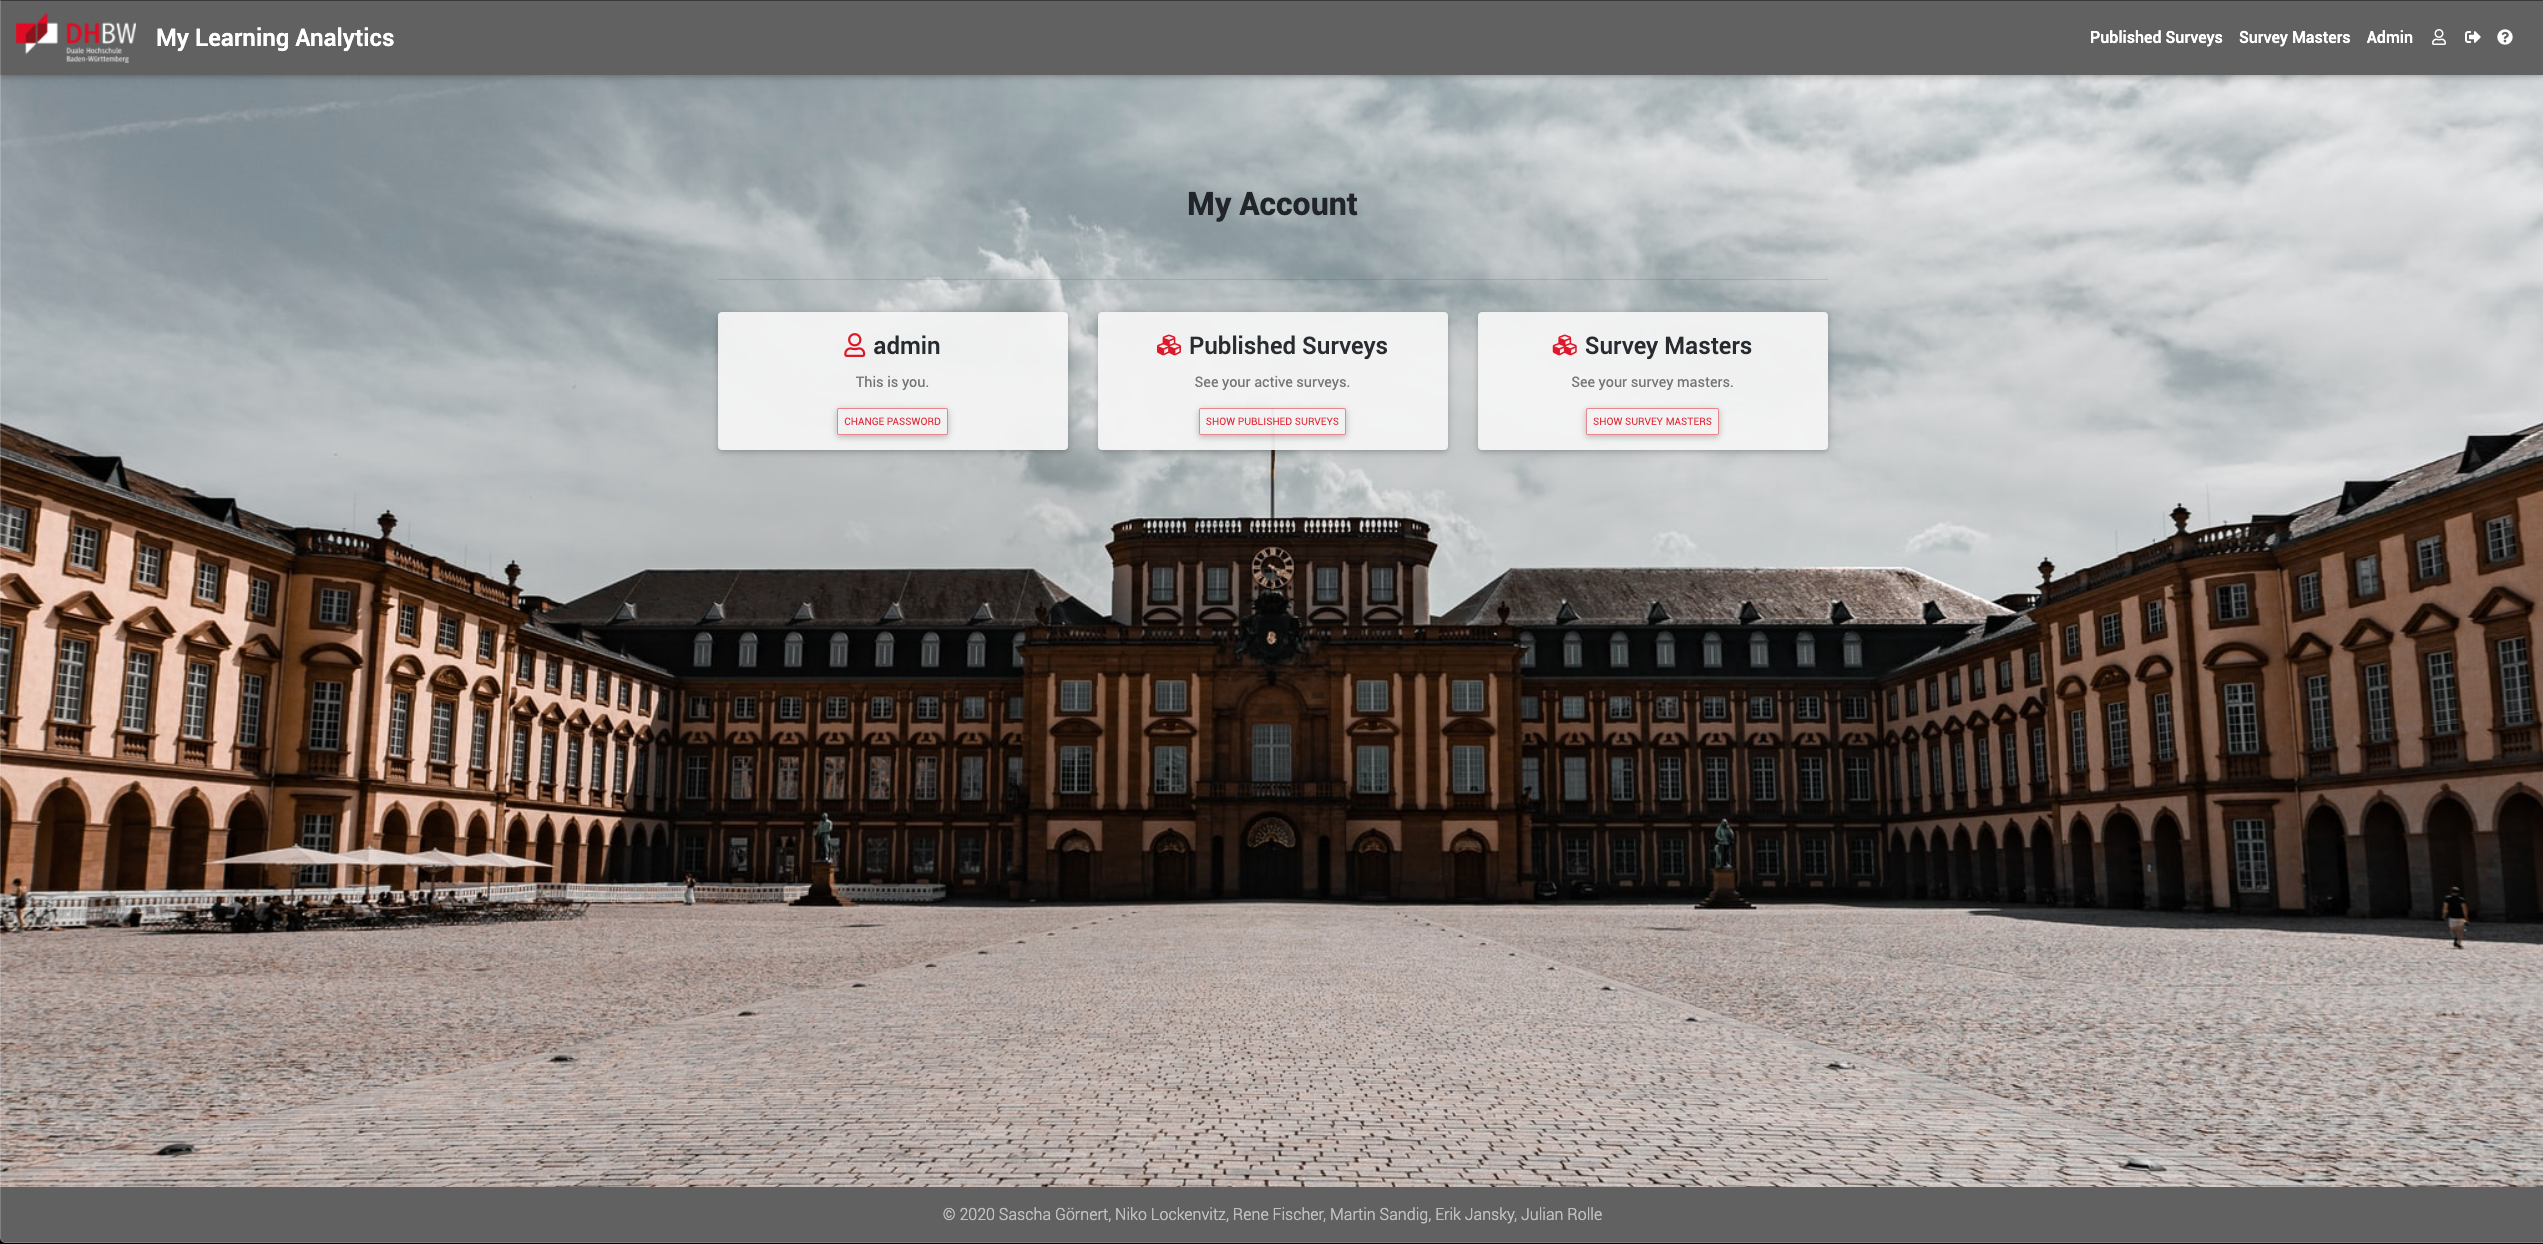
\includegraphics[width=0.95\textwidth, keepaspectratio]{img/client/Account.png}
	\captionsetup{justification=centering, format=plain}
	\caption[\acf{UI}: Benutzerkonto]{\acf{UI}: Benutzerkonto \\ \quelleScreenshot}
	\label{fig:AccountImplement}
\end{figure}


